%preamble
\documentclass[letterpaper]{article}
\synctex=1

\usepackage{geometry}
\usepackage{array}
\usepackage{lipsum}

\usepackage{graphicx}
\usepackage{float}
\graphicspath{ {images/} }

\usepackage{float}

\usepackage[hidelinks]{hyperref}

\usepackage{xcolor}
% \usepackage[section]{placeins}
%
% \newenvironment{changemargin}[2]{%
% \begin{list}{}{%
% \setlength{\topsep}{0pt}%
% \setlength{\leftmargin}{#1}%
% \setlength{\rightmargin}{#2}%
% \setlength{\listparindent}{\parindent}%
% \setlength{\itemindent}{\parindent}%
% \setlength{\parsep}{\parskip}%
% }%
% \item[]}{\end{list}}

% \usepackage{tabu}
%actual document
\begin{document}

%titlepage
\begin{titlepage}
 \begin{center}

  \LARGE
  ECE 321 Lab\\ Software Requirements Engineering
  
  Department of Electrical and Computer Engineering\\
  
  University of Alberta
  
  \vspace{2cm}
  
  404 Team Name Not Found
  
  \vspace{5cm}
  \Large
  
  \begin{tabular}{ | m{5cm} | m{5cm} | }
   \hline
   Student Name  & Student \\
   \hline
   Arun Woosaree & XXXXXX  \\
   \hline
   Max           & XXXXXX  \\
   \hline
   Liyao         & XXXXXX  \\
   \hline
  \end{tabular}
  
  
  % \begin{tabu} to 0.8\textwidth{  | X[c] | X[c] | }
  %   \hline
  %   Student Name & Student \\
  %   \hline
  %   Arun Woosaree & xxxxxxx \\
  %   \hline
  %   Navras Kamal & 1505463 \\
  %   \hline
  % \end{tabu}
  
  
 \end{center}
\end{titlepage}

%table of contents
\tableofcontents
\vfill
\newpage

\section{Customer:}
Client:
Alberta Traffic Supply Ltd.\\
7798 16 th Street\\
Edmonton, Alberta, T6P 1L9\\
Western Canada largest traffic sign manufacture and traffic control company\\

\section{Definitions}
\label{Definitions}
\begin{figure}[h!]
 \centering
 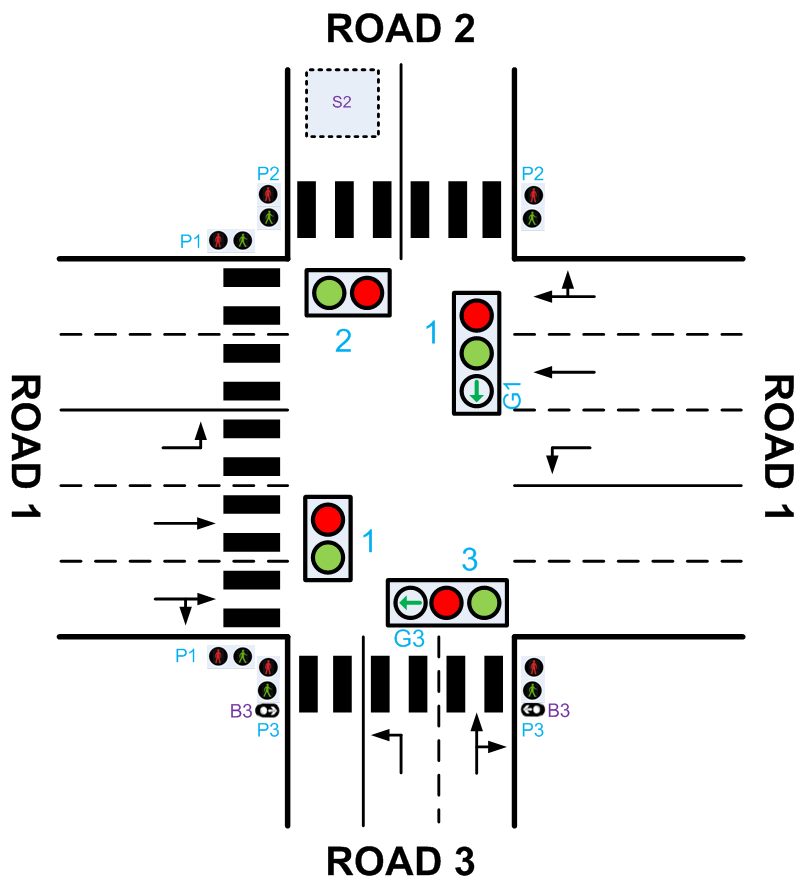
\includegraphics[width=\textwidth]{intersection.png}
 \caption{INSERT CAPTION HERE}
 \label{intersection}
\end{figure}

\textit{Labels}
\textbf{1,2,3,P1,P2,P3,B3,S2,G1,G3}
\textit{can be found in Figure \ref{intersection}.}
\begin{enumerate}

 \item \textbf{TLMS} -
       \textbf{T}raffic
       \textbf{L}ight
       \textbf{M}onitoring
       \textbf{S}ystem
       
 \item \textbf{RB} -
       \textbf{R}eset
       \textbf{Button}
 \item \textbf{M} - Hardware malfunction: 1 indicates a malfunction, 0 for normal operation
 \item \textbf{1} - Light on Road 1
 \item \textbf{2} - Light on Road 2
 \item \textbf{3} - Light on Road 3
 \item \textbf{P1} - Pedestrian light on road 1
 \item \textbf{P2} - Pedestrian light on road 2
 \item \textbf{P3} - Pedestrian light on road 3
 \item \textbf{t1} - Timer for \textbf{1}
 \item \textbf{t2} - Secondary timer for everything else
 \item \textbf{G1} - Left turn signal on road 1
 \item \textbf{G3} - Left turn signal on road 3
 \item \textbf{S2} - Magnetic sensor which detects if a car/motorcycle is waiting on \textbf{2}\\
       Outputs: 1 if vehicle waiting, 0 otherwise
 \item \textbf{B3} - Button on road 3 which a pedestrian can hit to request to cross the intersection
 \item \textbf{BG} -
       \textbf{B}linking
       \textbf{G}reen
 \item \textbf{BR}
       \textbf{B}linking
       \textbf{R}ed
 \item \textbf{D} - \textbf{D}ay
 \item \textbf{N} - \textbf{N}ight
 \item \textbf{Clock} - Can have value \textbf{D} or \textbf{N}
 \item \textbf{}
 \item \textbf{}
       
       
\end{enumerate}


\section{Description}
Lorem ipsum dolor sit amet, consectetur adipiscing elit, sed do eiusmod tempor
incididunt ut labore et dolore magna aliqua. Ut enim ad minim veniam, quis
nostrud exercitation ullamco laboris nisi ut aliquip ex ea commodo consequat.
Duis aute irure dolor in reprehenderit in voluptate velit esse cillum dolore eu
fugiat nulla pariatur. Excepteur sint occaecat cupidatat non proident, sunt in
culpa qui officia deserunt mollit anim id est laborum.
road \textbf{1} is main, \textbf{3} is also main but \textbf{1} is the most important, and
road \textbf{2} is secondary


\section{Requirements}
\begin{enumerate}
 \item yooo
\end{enumerate}

\section{Nice-to-haves}
\begin{enumerate}
 \item yooo
\end{enumerate}



\section{State description}
\textit{Labels}
\textbf{1,2,3,P1,P2,P3,B3,S2,G1,G3}
\textit{are defined on page \pageref{Definitions} and in Figure \ref{intersection} on page \ref{intersection}.}
\begin{enumerate}
 \item \textbf{Default}
       \begin{itemize}
        \item {\color{green}\textbf{1,P2}}
        \item {\color{red}\textbf{2,3,P1,P3,G1,G3}}
        \item \textbf{t1} activated
        \item \textbf{M}: 0
        \item \textbf{Clock}: \textbf{D}
       \end{itemize}
 \item \textbf{Green G1}
       \begin{itemize}
        \item {\color{green}\textbf{G1,P1}}
        \item {\color{red}\textbf{1,2,3,P2,P3,G3}}
        \item \textbf{t2} activated
        \item \textbf{M}: 0
        \item \textbf{Clock}: \textbf{D}
       \end{itemize}
       Notes:
       \begin{enumerate}
        \item \textbf{Green 3 S2} \textit{is this state, but when} \textbf{S2}=1
       \end{enumerate}
       
       
 \item \textbf{Green 3}
       \begin{itemize}
        \item {\color{green}\textbf{3,G3}}
        \item {\color{red}\textbf{1,2,P1,P2,P3,G1}}
        \item \textbf{t2} activated
        \item \textbf{M}: 0
        \item \textbf{Clock}: \textbf{D}
       \end{itemize}
       Notes:
       \begin{enumerate}
        \item \textbf{Green 3 S2} \textit{is this state, but when} \textbf{S2}=1
       \end{enumerate}
 \item \textbf{Green P3}
       \begin{itemize}
        \item {\color{green}\textbf{1,P2,P3}}
        \item {\color{red}\textbf{2,3,P1,G1,G3}}
        \item \textbf{t2} activated
        \item \textbf{M}: 0
        \item \textbf{Clock}: \textbf{D}
       \end{itemize}
       Notes:
       \begin{enumerate}
        \item \textbf{Green 3 S2} \textit{is this state, but when} \textbf{S2}=1
       \end{enumerate}
 \item \textbf{Green 2\&3}
       \begin{itemize}
        \item {\color{green}\textbf{2,3}}
        \item {\color{red}\textbf{1,P1,P2,P3,G1,G3}}
        \item \textbf{t2} activated
        \item \textbf{M}: 0
        \item \textbf{Clock}: \textbf{D}
       \end{itemize}
 \item \textbf{Night}
       \begin{itemize}
        \item {\color{green}\textbf{1}} \textbf{BG}
        \item {\color{red}\textbf{2,3}} \textbf{BR}
        \item \textbf{P1,P2,P3,G1,G3} are turned off
        \item \textbf{M}: 0
        \item \textbf{Clock}: \textbf{N}
       \end{itemize}
 \item \textbf{Emergency}
       \begin{itemize}
        \item {\color{green}\textbf{1}} \textbf{BG}
        \item {\color{red}\textbf{2,3}} \textbf{BR}
        \item \textbf{P1,P2,P3,G1,G3} are turned off
        \item \textbf{M}: 1
        \item \textbf{Clock}: \textbf{D} or \textbf{N}
       \end{itemize}
\end{enumerate}

\begin{figure}[H]
 \centering
 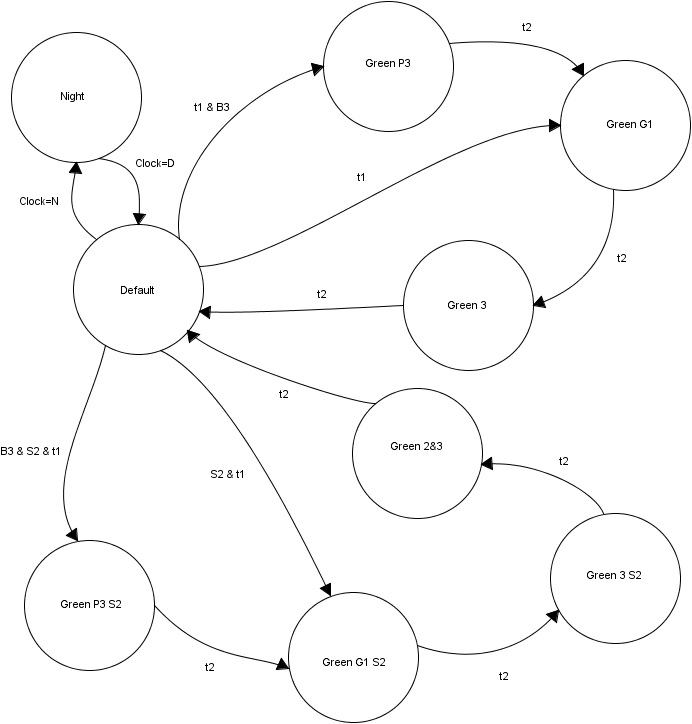
\includegraphics[width=\textwidth]{fsm.png}
 \caption{INSERT CAPTION HERE}
 \label{fsm}
\end{figure}

\section{Special considerations}

\begin{enumerate}
 \item Security\\
       Here's how we make the system more secure:
       \begin{enumerate}
        \item step 1
        \item step 2
        \item step 3
       \end{enumerate}
 \item Reliability
 \item Synced timings
\end{enumerate}


\end{document}
